\documentclass[a4paper]{report}

\usepackage{textcomp}
\usepackage{graphicx}
\usepackage{parskip}
\usepackage{hyperref}
\usepackage{color}
\usepackage{verbatim}
\usepackage[usenames,dvipsnames,svgnames,table]{xcolor}
\usepackage{tikz}
\usepackage{tikz-uml}
\usepackage{pdfpages}


\usepackage[T1]{fontenc}
\usepackage[utf8]{inputenc}
\usepackage[english]{babel}
\usepackage{listings}

\lstdefinelanguage{tikzuml}{language=[LaTeX]TeX, classoffset=0, morekeywords={umlbasiccomponent, umlprovidedinterface, umlrequiredinterface, umldelegateconnector, umlassemblyconnector, umlVHVassemblyconnector, umlHVHassemblyconnector, umlnote, umlusecase, umlactor, umlinherit, umlassoc, umlVHextend, umlinclude, umlstateinitial, umlbasicstate, umltrans, umlstatefinal, umlVHtrans, umlHVtrans, umldatabase, umlmulti, umlobject, umlfpart, umlcreatecall, umlclass, umlvirt, umlunicompo, umlimport, umlaggreg}, keywordstyle=\color{DarkBlue}, classoffset=1, morekeywords={umlcomponent, umlsystem, umlstate, umlseqdiag, umlcall, umlcallself, umlfragment, umlpackage}, keywordstyle=\color{DarkRed}, classoffset=0,  sensitive=true, morecomment=[l]{\%}}

\begin{document}

\begin{titlepage}
			\begin{center}
			\textsc{\LARGE {IN3405 Bachelor Project}}\\[1cm]
			\rule{\linewidth}{0.5mm} \\[0.4cm]

			{\Huge \bfseries NAME}\\[0.15cm]

			\rule{\linewidth}{0.5mm} \\[1.5cm]
			
			\vskip 2 cm
			
\includegraphics[scale=0.5]{title.jpg}
			\vskip 1 cm
				\rule{\linewidth}{0.5mm}
			
			\vskip 0.5 cm
			
			\begin{minipage}{0.4\textwidth}
				\begin{flushleft} \large
					\emph{Authors:}\\
					\begin{tabular}{l}
						S.E. Austin (4005996) \\
						A. Drif (4030532) \\
						W.K.H. Ko (4005686) \\
						J.E.T. Tan (4032918)
					\end{tabular}
				\end{flushleft}
			\end{minipage}
			\hspace{1cm}
			\begin{minipage}{0.4\textwidth}
				\begin{flushright} \large
					\emph{Supervisor:} \\
					Dr.Ir. J.A. Pouwelse
				\end{flushright}
			\end{minipage}
			
			\vskip 0.5 cm
			
			\rule{\linewidth}{0.5mm}
			\end{center}
\end{titlepage}

\chapter*{Preface}
In the third year of the Computer Science course in Delft, students have to do their Bachelor project, 
where they have to work under supervision of a professor.

This report is part of our Bachelor Project, carried out in the academic year 2011-2012. The goal of this project is to develop a 4th generation peer-to-peer application to be used on a Samsung Smart TV.

We would like to thank our supervisor and the Tribler team, which helped us with this project.

\tableofcontents

\chapter*{Summary}
Since their invention, TV\textquotesingle s have become one of the most popular media devices and can be found in almost every livingroom in the 
world. For a long time, the functionality of the TV stayed the same: the ability to view television programs at certain fixed times of the day.
Recently there has been development in the television market adding computing power and internet connectability to televisions.
These new features open a whole new world of possibilities.

The goal of this project was to create an application that runs on a Samsung SmartTV and uses the libswift peer-to-peer engine to download, upload 
and stream files. To create an application for a Samsung SmartTV a software development kit has been provided which allows programmers to create 
apps using JavaScript, HTML, CSS and Flash. This software development kit was used to create the front-end of our application. 
The front-end consists of an internal media player to handle streaming content and media playback found
 on an external USB device.

A Samsung SmartTV runs a linux kernel in which we can properly run our download-engine which is written in C++.
To be able to do this we gained root access to the TV, so it became possible to operate in the linux environment. After this was done, the back-end for our application was implemented in C++. In order to make the front-end communicate with the back-end, we used the client-server architecture where the front-end acts as a client and the back-end as a server.

It was also needed to provide a communication mechanism between TV\textquotesingle s, so that content could be found and shared between TV\textquotesingle s. This was achieved by using the Dispersy and DHT modules developed by the
tribler team. These modules were, however, implemented in Python. In order to make use of this, a part of our application is implemented in Python.

Several steps were taken in order to develop this application. An analysis of requirements was made, which serves as the foundation of the design
of our application. A design following the client-server pattern was made, after which class and sequence diagrams were created.

During development we encountered a lot of problems, mostly because the TV runs a stripped version of the linux kernel. The consequence was that a
lot of things were not available on the TV, so we had to cross-compile the necessities for the TV or use a binary compatible development platform. 
Other problems we encountered were for example that the TV sends TCP RST packages to itself. Also, problems during implementation occured when we 
used threads for the implementation of the HTTP server.

Even though we encountered these problems, we were still able to maintain our schedule and develop everything in time.
By doing several things together and by dividing the work correctly we were able to overcome the mentioned problems.
 The result is the first fourth generation peer-to-peer application in the world running natively on a Samsung SmartTV.
 Even though this is an achievement we are proud of, the application is still a proof of concept since current TV\textquotesingle s are not strong enough to run the application smoothly.
 This might change in the future, when TV\textquotesingle s become more powerful.

\chapter{Introduction}
The client, but also supervisor of this project is Dr.Ir. Johan Pouwelse from the Parallel and Distributed Systems group on the faculty of EEMCS of the Delft University of Technology.
He is the scientific director of several peer-to-peer research initiatives and also the founder and leader of the Tribler peer-to-peer research team.
Tribler\cite{tribler} is an open source peer-to-peer client that is completely decentralised.
The application to be implemented is required to have the same download-engine, swift,\cite{swift} as Tribler
along with an internal media player to handle streaming content and possibly media playback found on an external USB device.

Libswift is a lightweight 4th generation peer-to-peer based transport protocol for content dissemination
that can run on top of other protocols, such as UDP, TCP, HTTP, or as RTP profile.
It can be used for both live streaming and conventional downloading purposes.
4th generation peer-to-peer software means that it is fully self-organised, removing the need for any server\footnote{\url{http://www.tribler.org/trac/wiki/4thGenerationP2P}}.

Because swift is a very generic protocol, it should be easy to merge with the existing technology of the TV.
Since the Smart TV has limited memory and CPU resources, 
it is necessary that the application to be build is as lightweight as possible.
The streaming capabilities also enables the user to maximise utility of the TV,
while still able to download data and store it.
A major drawback is however that downloading and streaming content is limited to the memory of the TV.
% Drawback is niet nodig hier in de inleiding, komt later aan de orde en meteen ook vermelden dat tv's steeds sterker worden
% Hier ook vertellen dat: 
%het een proof of concept is, 
%p2p tv zonder devices aan te sluiten op de tv(behalve usb),

\chapter{Problem Statement}
\label{sec:problems}
The goal of this project is to create an application that runs on a Samsung SmartTV and uses the libswift peer-to-peer engine to download, upload and stream files. To create an application for a Samsung SmartTV\footnote{\url{http://www.samsung.com/nl/experience/tv/smarttv/}} a software development kit has been provided which allows programmers to create apps using JavaScript, HTML, CSS and Flash (See \hyperref[sec:terms]{terms of reference}).\\\\
A Samsung SmartTV however runs a linux kernel in which we can properly run our download-engine which is written in C++. To be able to do this we must gain root access to the TV, so it becomes possible to operate in the linux environment (See also \hyperref[sec:orientation]{orientation report}). A problem that arises here is that the SDK front-end will be completely separated from the back-end where libswift will run. A solution has to be found to escape from this sandboxed environment. It is also needed to provide a communication mechanism between TV\textquotesingle s,
so that content can be found and shared between TV\textquotesingle s.

Problems to be solved
\begin{itemize}
\item Root a Samsung television
\item Create a C++ back-end with swift
\item Break out of the sandbox
\item Create a JavaScript front-end
\item Inter-TV communication
\end{itemize}

This application will be a proof of concept to show that televisions are capable of running peer-to-peer software natively, without any attached
devices, in this case with the help of the libswift download-engine. Therefore usability is not the primary goal of this application, 
although the application will be designed to be as usable as possible.

\chapter{Requirements Analysis}

This chapter discusses the design process of our application. First, it was needed to know what the user requirements are. For this, we interviewed our supervisor who also acts as our client. These requirements were also acquired through brainstorming. Then, use cases for our application were designed, which corresponds with the user requirements. In this phase, a business class diagram was also made which is easier to understand for the client than the complete class diagram of the whole application. After researching the framework present on the Samsung Smart TV and the possibilities of libswift, a design for the software architecture could be made. Lastly, implementation models such as sequence diagrams and class diagrams were made, which serve as blueprints for the application.

\section{Requirements}
The requirements can be split in two kinds, functional and non-functional requirements. These requirements  correspond to the use cases as mentioned in section \hyperref[sec:use_cases]{\ref*{sec:use_cases}} The non-functional requirements can then again be split in quality and platform requirements. In this section, the constraints the application has to deal with are also discussed.

\subsection{Functional requirements} 
Functional requirements specify the core functionality of the application. These requirements are covered by the use cases in the next section. The functional requirements are as follows:

\begin{itemize}
\item[1.] Given two peers \textit{A} and \textit{B}:
	\begin{itemize}
	\item[1.1.] \textit{A} is able to download from \textit{B} (UC 12);
	\item[1.2.] \textit{A} is able to upload to \textit{B} (Should happen automatically after download is finished);
	\item[1.3.] \textit{A} is able to stream to/from \textit{B} (UC 11);
	\end{itemize}	
\item[2.] The users should be able to search for files other peers own (UC 9, 10);
\item[3.] The users should be able to search/browse files they own themselves (UC 2, 8, 10);
\item[4.] The users should be able to playback media content. 
		  Media in this context means any kind of video or audio file (UC 6);
\item[5.] Users should be able to:
	\begin{itemize}
	\item[5.1.] Move files on the file system (UC 5);
	\item[5.2.] Edit files on the file system, i.e. rename files (UC 3);	
	\item[5.3.] Remove files on the file system (UC 4);
	
	\end{itemize}
\item[6.] Users should be able to sort files by name, size, date and type (UC 13, 14, 15, 16, 17); 
\item[7.] Users should be able to separate private files from public files (UC 7);
\item[8.] Users should be able to limit the upload/download speed (UC 1). 
\end{itemize} 

\subsection{Non-functional requirements}
Non-functional requirements are those requirements that have to do with the operation of the system. 
Unlike functional requirements, they do not describe what the services the system should provide, 
but more how the system should work. We identified two kinds of non-functional requirements for our application, 
quality and platform requirements.

\subsubsection{Quality requirements}
\begin{itemize}
\item[9.] The response time of the system should be as low as possible since TVs are real-time systems.
We aim to limit the response time to 300 ms;
\item[10.] The RAM memory used by the application should not exceed 256 MB.
This includes the size of the application itself and the memory needed for calculations;
\item[11.] The application may use 100\% CPU power since no other applications should run along the application 
to be built;
\item[12.] Downloads should be continued without loss of data after a failure;
\item[13.] Unfinished downloads should be resumed at start up;
\item[14.] The application should be able to cope with external devices,
memory sticks and other external storage devices in particular;
\item[15.] The user should be able to make use of (part of) the application at any time,
even when no Internet connection is available.
\end{itemize}

\subsubsection{Platform requirements}
\begin{itemize}
\item[1.] The C++ back-end which makes use of the libswift library should be implemented so 
that it is reusable for other systems that work with other front-ends (such as Android);
\item[2.] The application is made to run on a rooted Samsung Smart TV.
To see whether a Samsung TV is rootable or not, please check \url{http://www.samygo.tv/};
\end{itemize}

\subsection{Constraints}
The constraints specify what our own limitations are we have to take into account when implementing the application. 
These can be limitations put by the software we use, 
or put by ourselves to reduce the application\textquotesingle s complexity.

\begin{itemize}
\item[1.] Due to the limited memory available on the TV, it is not 
possible to download and store great amounts of data on the TV. 
Therefore, usage of external storage devices is mandatory to make use 
of the application;

\item[2.] The application must be integrated with the Samsung 
framework, meaning that it should be recognised by the TV as 
JavaScript app developed with the Samsung SDK.
\end{itemize}

\section{Use Cases}
\label{sec:use_cases}
The use case models describe interactions between one or more actors and the system. 
The models are used to depict what the users can do with the system and how they  should operate it.
In our case, we only have one actor, which is the user who watches TV. This is because our application should always
maintain the same behaviour for everyone who uses it; everyone using the application has the same rights, privileges 
and use cases of the system. The use cases are shown in figure \ref{fig:use_case_diagram}, 
in which the relations between them are also shown. The user should be able to carry out all the use cases, 
these relations are left out for clarity. The use cases in figure \ref{fig:use_case_diagram} 
are explained in further detail in their descriptions and with the use of UML sequence diagrams in sections 
\hyperref[sec:use_case_descriptions]{\ref*{sec:use_case_descriptions}} and 
\hyperref[sec:req_dynamic_models]{\ref*{sec:req_dynamic_models}} respectively.

\begin{center}
\begin{figure}[h!]
\begin{tikzpicture}
\begin{umlsystem}[fill=red!10]{The system}

\umlusecase[x=6, width=4cm]{1.Limit upload/download speed}
\umlusecase[x=-2, y=-4, width=1.5cm]{3.Update Files}
\umlusecase[x=1, y=-3, width=1.5cm]{4.Delete Files}
\umlusecase[x=7, y=-2, width=3cm]{6.Play Media File}
\umlusecase[width=3cm]{2.Browse File System}
\umlusecase[x=4, y=-4, width=1.5cm]{5.Move Files}
\umlusecase[x=7, y=-9, width =1.5cm]{11.Stream File}
\umlusecase[x=7, y=-11, width =1.5cm]{12.Download File}
\umlusecase[x=8, y=-4, width=3cm]{7.Change File Visibility}
\umlusecase[y=-10, width=1.5cm]{13.Sort Files}
\umlusecase[x=-1, y=-7, width=1.5cm]{8.Search locally}
\umlusecase[x=2, y=-7, width=1.5cm]{9.Search on the net}
\umlusecase[x=3, y=-10, width=1.5cm]{10.Search File}
\umlusecase[x=-2, y=-14, width=1.5cm]{14.Sort by date}
\umlusecase[x=0, y=-14, width=1.5cm]{15.Sort by type}
\umlusecase[x=2, y=-14, width=1.5cm]{16.Sort by name}
\umlusecase[x=4, y=-14, width=1.5cm]{17.Sort by size}

\end{umlsystem}

\umlactor[x=-4.5, y=-5]{User}

\umlinclude[name=incl]{usecase-7}{usecase-12}
\umlinclude[name=incl]{usecase-8}{usecase-12}

\umlinclude[name=incl]{usecase-9}{usecase-5}
\umlinclude[name=incl]{usecase-2}{usecase-5}
\umlinclude[name=incl]{usecase-3}{usecase-5}
\umlinclude[name=incl]{usecase-4}{usecase-5}
\umlinclude[name=incl]{usecase-6}{usecase-5}
\umlHVinclude[name=incl]{usecase-10}{usecase-5}
\umlVHinclude[name=incl]{usecase-4}{usecase-11}

\umlinclude[name=incl]{usecase-2}{usecase-11}
\umlinclude[name=incl]{usecase-3}{usecase-11}
\umlinclude[name=incl]{usecase-6}{usecase-11}
\umlinclude[name=incl]{usecase-9}{usecase-11}

\umlVHVinherit{usecase-14}{usecase-10}
\umlVHVinherit{usecase-15}{usecase-10}
\umlVHVinherit{usecase-16}{usecase-10}
\umlVHVinherit{usecase-17}{usecase-10}

\umlVHVinherit{usecase-11}{usecase-13}
\umlVHVinherit{usecase-12}{usecase-13}

\end{tikzpicture}
\label{fig:use_case_diagram}
\caption{Use case diagram of the application to be built. 
Note that the associations from the user to the use cases are left out in order to keep the diagram clear.}
\end{figure}
\end{center}

\clearpage
\subsection{Use Case Descriptions}
\label{sec:use_case_descriptions}

\begin{table}[h!]
\centering
\begin{tabular}{|l|l|}
\hline
Name & Limit upload/download speeds\\ \hline
Goal & Save bandwidth.\\ \hline
Preconditions & -- \\ \hline
Summary & The user adjusts the upload or download speed.\\ \hline
Steps &  1. User clicks the settings button; \\
      &  2. \textit{System} shows the settings page; \\
      &  3. User sets the download and upload speeds; \\
      &  4. User clicks OK button; \\
      &  5. \textit{System} saves the settings and applies the new speeds;
        \\ \hline
Postconditions & Downloads and uploads will never exceed the new speeds.
\\ \hline
\end{tabular}
\caption{Use Case 1: Limit upload/download speeds}
\label{tab:UC1}
\end{table}

\begin{table}[h!]
\centering
\begin{tabular}{|l|l|}
\hline
Name & Browse File System\\ \hline
Goal & Getting an overview of the files in the file system.\\ \hline
Preconditions & One or more external storage devices are connected. \\ \hline
Summary & The user browses through the directories on the file system.\\ \hline
Related Cases & Play Media File, Move File, Update File, Delete File, \\ 
              &  Sort Files, Change File Visibility. \\ \hline
Steps &  1. User selects the device to browse; \\
      &  2. \textit{System} shows list of files and directories of the selected device. 
        \\ \hline
Postconditions & Downloads and uploads will never exceed the new speeds.
\\ \hline
\end{tabular}
\caption{Use Case 2: Browse File System}
\label{tab:UC2}
\end{table}

\begin{table}[h!]
\centering
\begin{tabular}{|l|l|}
\hline
Name & Update Files\\ \hline
Goal & Change the properties of a file.\\ \hline
Preconditions & A changeable file is available locally. \\ \hline
Summary & The user changes the properties of a local file.\\ \hline
Related Cases & Includes \textbf{Browse File System} and \textbf{Search locally}. \\ \hline
Steps &  1. User selects the file to update; \\
      &  2. \textit{System} shows the properties of the file; \\ 
      &  3. User changes the properties and clicks the OK button; \\
      &  4. \textit{System} changes the properties and saves them. 
        \\ \hline
Postconditions & File properties are changed locally and if uploading, also online.
\\ \hline
\end{tabular}
\caption{Use Case 3: Update Files}
\label{tab:UC3}
\end{table}

\begin{table}[h!]
\centering
\begin{tabular}{|l|l|}
\hline
Name & Delete Files\\ \hline
Goal & Delete one or more files.\\ \hline
Preconditions & A deletable file is available locally. \\ \hline
Summary & The user deletes a file.\\ \hline
Related Cases & Includes \textbf{Browse File System} and \textbf{Search locally}. \\ \hline
Steps &  1. User selects the files to delete; \\
      &  2. \textit{System} asks for confirmation; \\ 
      &  3. User clicks the OK button; \\
      &  4. \textit{System} deletes selected files. 
        \\ \hline
Postconditions & Files are deleted locally and if uploading, also online.
\\ \hline
\end{tabular}
\caption{Use Case 4: Delete Files}
\label{tab:UC4}
\end{table}

\begin{table}[h!]
\centering
\begin{tabular}{|l|l|}
\hline
Name & Move Files\\ \hline
Goal & Move one, multiple files or directories.\\ \hline
Preconditions & A moveable file or directory is available locally. \\ \hline
Summary & The user selects files or directories and moves them in the file system.\\ \hline
Related Cases & Includes \textbf{Browse File System} and \textbf{Search locally}. \\ \hline
Steps &  1. User selects the files or directories to move; \\
      &  2. User browses to the new location; \\
      &  3. \textit{System} moves the selected files and directories. 
        \\ \hline
Postconditions & Files are moved to another directory.
\\ \hline
\end{tabular}
\caption{Use Case 5: Move Files}
\label{tab:UC5}
\end{table}

\begin{table}[h!]
\centering
\begin{tabular}{|l|l|}
\hline
Name & Play Media File\\ \hline
Goal & Play a music or video file or display a picture.\\ \hline
Preconditions & A playable file is available. \\ \hline
Summary & The user opens a stream or a locally available file.\\ \hline
Related Cases & Includes \textbf{Browse File System} and \textbf{Search locally}. \\ \hline
Steps &  1. User selects the file to play; \\
      &  2. \textit{System} either starts the photo viewer or media player to open the file. 
        \\ \hline
Postconditions & File is opened and is viewable/listenable.
\\ \hline
\end{tabular}
\caption{Use Case 6: Play Media File}
\label{tab:UC6}
\end{table}

\begin{table}[h!]
\centering
\begin{tabular}{|l|l|}
\hline
Name & Change File Visibility\\ \hline
Goal & Start or stops the uploading of a file.\\ \hline
Preconditions & An uploadable file is available. \\
& Also, the system must be connected to the Internet. \\ \hline
Summary & The user checks/unchecks the visibility box \\
& of a file to control file uploads.\\ \hline
Related Cases & Includes \textbf{Browse File System} and \textbf{Search locally}. \\ \hline
Steps &  1. User checks or unchecks the visibility box of a file; \\
      &  2. \textit{System} either starts uploading the file and adds the upload to the Upload \\
      &     Manager or  stops uploading the file and removes the upload from the Upload \\
      &     Manager.
        \\ \hline
Postconditions & File is uploaded or removed from the Upload Manager.
\\ \hline
\end{tabular}
\caption{Use Case 7: Change File Visibility}
\label{tab:UC7}
\end{table}

\begin{table}[h!]
\centering
\begin{tabular}{|l|l|}
\hline
Name & Search locally\\ \hline
Goal & Find a file on an external storage device.\\ \hline
Preconditions & One or more external storage devices are connected. \\ \hline
Summary & The user searches with keywords for files in a file system.\\ \hline

Related Cases & Play Media File, Move File, Update File, Delete File, \\ 
              & Change File Visibility. Inherits \textbf{Search File} \\ \hline
Steps &  1. User presses Search button; \\
      &  2. \textit{System} shows Search menu; \\
      &  3. User sets search range on ``Local''; \\
      &  4. User selects the file type to search; \\
      &  5. User puts keywords in the textbox and presses Start button; \\
      &  6. \textit{System} returns with a list and number of found files. 
        \\ \hline
Postconditions & A list of found files is returned together with the number of found files.
\\ \hline
\end{tabular}
\caption{Use Case 8: Search locally}
\label{tab:UC8}
\end{table}

\begin{table}[h!]
\centering
\begin{tabular}{|l|l|}
\hline
Name & Search on the net\\ \hline
Goal & Find a file to download or stream on the Internet.\\ \hline
Preconditions & The system is connected to the Internet. \\ \hline
Summary & The user searches with keywords for media content on the Internet.\\ \hline

Related Cases & Stream File, Download File. Inherits \textbf{Search File} \\ \hline
Steps &  1. User presses Search button; \\
      &  2. \textit{System} shows Search menu; \\
      &  3. User sets search range on ``Online''; \\
      &  4. User selects the file type to search; \\
      &  5. User puts keywords in the textbox and presses Start button; \\
      &  6. \textit{System} returns with a list and number of found files. 
        \\ \hline
Postconditions & A list of found files is returned together with the number of found files.
\\ \hline
\end{tabular}
\caption{Use Case 9: Search on the net}
\label{tab:UC9}
\end{table}

\begin{table}[h!]
\centering
\begin{tabular}{|l|l|}
\hline
Name & Search File\\ \hline
Goal & Find a file by using keywords.\\ \hline
Preconditions & A keyword with length > 0 is provided by the user. \\ \hline
Summary & The user searches for a file.\\ \hline
Related Cases & Generalizes \textbf{Search locally} and \textbf{Search on the net}. \\ \hline
Steps &  1. User inputs a keyword; \\
      &  2. User selects the file type to search; \\
      &  3. \textit{System} returns the list and number of found files. 
        \\ \hline
Postconditions & A list and number of found files is returned.
\\ \hline
\end{tabular}
\caption{Use Case 10: Search File}
\label{tab:UC10}
\end{table}

\begin{table}[h!]
\centering
\begin{tabular}{|l|l|}
\hline
Name & Stream File\\ \hline
Goal & Listen to a stream and play its content.\\ \hline
Preconditions & A network connection is established. \\
& Also, an external storage device must be connected. \\ \hline
Summary & The user plays the content of a stream. \\
& This can happen either online or within the local network.\\ \hline

Related Cases & Includes \textbf{Search on the net}. \\ \hline
Steps &  1. Selects an uploaded file; \\
      &  2. \textit{System} shows options ``Download'' and ``Open''; \\
      &  3. User selects ``Open''; \\
      &  4. \textit{System} starts the videoplayer and plays the stream.
        \\ \hline
Postconditions & A stream is opened and played by the videoplayer. \\
& Temporary files are removed after playing the stream.
\\ \hline
\end{tabular}
\caption{Use Case 11: Stream File}
\label{tab:UC11}
\end{table}

\begin{table}[h!]
\centering
\begin{tabular}{|l|l|}
\hline
Name & Download File\\ \hline
Goal & Download a file and puts it in the file system.\\ \hline
Preconditions & A network connection is established. \\
& Also, an external storage device must be connected. \\ \hline
Summary & The user plays the content of a stream. \\
& This can happen either online or within the local network.\\ \hline

Related Cases & Includes \textbf{Search on the net}. \\ \hline
Steps &  1. Selects an uploaded file; \\
      &  2. \textit{System} shows options ``Download'' and ``Open''; \\
      &  3. User selects ``Download''; \\
      &  4. \textit{System} adds the Download to the Download Manager and starts download.
        \\ \hline
Postconditions & A file is retrieved from the Internet and stored on the file system.
\\ \hline
\end{tabular}
\caption{Use Case 12: Download File}
\label{tab:UC12}
\end{table}

\begin{table}[h!]
\centering
\begin{tabular}{|l|l|}
\hline
Name & Sort Files\\ \hline
Goal & Arrange the files in a coherent way.\\ \hline
Preconditions & An external storage device is connected. \\ \hline
Summary & The user sorts the files.\\ \hline
Related Cases & Generalizes \textbf{Sort by type}, \textbf{Sort by name}, \\
& \textbf{Sort by date}, \textbf{Sort by size} . \\ \hline
Steps &  1. User clicks on attribute ``type'', ``name'', ``date'' or ``size''; \\
      &  2. \textit{System} sorts the files and returns the sorted list. 
        \\ \hline
Postconditions & A sorted list is returned.
\\ \hline
\end{tabular}
\caption{Use Case 13: Sort Files}
\label{tab:UC13}
\end{table}

\begin{table}[h!]
\centering
\begin{tabular}{|l|l|}
\hline
Name & Sort by date\\ \hline
Goal & Arrange the files by date.\\ \hline
Preconditions & An external storage device is connected. \\ \hline
Summary & The user sorts the files by date.\\ \hline
Related Cases & Inherits \textbf{Sort files}. \\ \hline
Steps &  1. User clicks on attribute ``date''; \\
      &  2. \textit{System} sorts the files by their dates of creation
      \\ & and returns the sorted list (ascending); \\
      &  3. User clicks on attribute ``date'' again; \\
      &  4. \textit{System} sorts the files by their dates of creation
      \\ & and returns the sorted list (descending).
        \\ \hline
Postconditions & A list sorted by date is returned.
\\ \hline
\end{tabular}
\caption{Use Case 14: Sort by date}
\label{tab:UC14}
\end{table}

\begin{table}[h!]
\centering
\begin{tabular}{|l|l|}
\hline
Name & Sort by type\\ \hline
Goal & Arrange the files by type.\\ \hline
Preconditions & An external storage device is connected. \\ \hline
Summary & The user sorts the files by type.\\ \hline
Related Cases & Inherits \textbf{Sort files}. \\ \hline
Steps &  1. User clicks on attribute ``type''; \\
      &  2. \textit{System} sorts the files by their types 
      \\ & and returns the sorted list (ascending); \\
      &  3. User clicks on attribute ``type'' again; \\
      &  4. \textit{System} sorts the files by their types
      \\ & and returns the sorted list (descending).
        \\ \hline
Postconditions & A list sorted by type is returned.
\\ \hline
\end{tabular}
\caption{Use Case 15: Sort by type}
\label{tab:UC15}
\end{table}

\begin{table}[h!]
\centering
\begin{tabular}{|l|l|}
\hline
Name & Sort by name\\ \hline
Goal & Arrange the files by name.\\ \hline
Preconditions & An external storage device is connected. \\ \hline
Summary & The user sorts the files by name.\\ \hline
Related Cases & Inherits \textbf{Sort files}. \\ \hline
Steps &  1. User clicks on attribute ``name''; \\
      &  2. \textit{System} sorts the files by their names
      \\ & and returns the sorted list (ascending); \\
      &  3. User clicks on attribute ``name'' again; \\
      &  4. \textit{System} sorts the files by their names
      \\ & and returns the sorted list (descending).
        \\ \hline
Postconditions & A list sorted by name is returned.
\\ \hline
\end{tabular}
\caption{Use Case 16: Sort by name}
\label{tab:UC16}
\end{table}

\clearpage

\begin{table}[t]
\centering
\begin{tabular}{|l|l|}
\hline
Name & Sort by size\\ \hline
Goal & Arrange the files by size.\\ \hline
Preconditions & An external storage device is connected. \\ \hline
Summary & The user sorts the files by size.\\ \hline
Related Cases & Inherits \textbf{Sort files}. \\ \hline
Steps &  1. User clicks on attribute ``size''; \\
      &  2. \textit{System} sorts the files by their sizes
      \\ & and returns the sorted list (ascending); \\
      &  3. User clicks on attribute ``name'' again; \\
      &  4. \textit{System} sorts the files by their sizes
      \\ & and returns the sorted list (descending).
        \\ \hline
Postconditions & A list sorted by size is returned.
\\ \hline
\end{tabular}
\caption{Use Case 17: Sort by size}
\label{tab:UC17}
\end{table}

\clearpage

\section{Business Class Diagram}

\begin{center}
\begin{figure}[h!]
\begin{tikzpicture}
%\begin{umlpackage}{p}
%\begin{umlpackage}{sp1}

\umlclass[x=-5]{Sendable}{
  - trackers : list<tracker> \\
  - seeders  : list<seeder> \\
  - speed	   : double
}{
  + stop() : void \\
  + pause() : void \\
}

\umlclass[x=3]{FileManager}{
  - list<File>
}{
  + remove(File file) : void \\
  + add(File file) : File \\
  + rename(File file) : File \\
  + sort() : void \\
  + search(File file) : list<File> \\
}

\umlclass[x=3, y=-6]{File}{
  - name : String \\
  - date : String \\
  - extension : String \\
  - size : double \\
  - visible : bool \\
}{
  + setVisibility(bool value) : void \\
  + isVisible() : bool \\
  + setName(String name) : void \\
  + getSize() : double \\
  + getDate() : String \\
  + getName() : String
}

\umlclass[x=4, y=-11]{Media}{
  - length : double \\
}{}

\umlclass[x=-7, y=-4]{Download}{
  - percentage : double
}{
  + start() : void \\
  + resume() : void
}

\umlclass[x=-3, y=-4]{Upload}{
  - amount : double
}{
  + start() : void \\
  + resume() : void
}

\umlclass[x=-5, y=-6]{Stream}{
  - amount : double
}{
  + play() : void
}

\umlclass[x=-5, y=-10.5]{DownloadManager}{
  - downloaded : double \\
  - uploaded : double \\
  - downloads : list<Download> \\
  - uploads : list<Uploads>
}{
  + startDownload(String link) : void \\
  + stopDownload(String link) : void \\
  + pauseDownload(String link) : void \\
  + resumeDownload(String link) : void \\
  + startUpload(String name) : void \\
  + stopUpload(String name) : void
}

\umlclass[x=2, y=-14]{MediaPlayer}{
}{
  + open(Media file) : void \\
  + open(Stream stream) : void
}

\umlaggreg[mult1=1, mult2=1, pos=0.8, angle1=30, angle2=60]{Sendable}{File}
\umlaggreg[mult1=1, mult2=*]{FileManager}{File}

\umlVHVinherit{Download}{Sendable}
\umlVHVinherit{Upload}{Sendable}
\umlinherit{Stream}{Sendable}

\umlVHVinherit{Media}{File}

\umlVHVaggreg[mult1=1, mult2=*]{DownloadManager}{Upload}
\umlVHVaggreg[mult1=1, mult2=*]{DownloadManager}{Download}

\umlVHassoc{MediaPlayer}{Stream}
\umlVHassoc{Media}{MediaPlayer}

\end{tikzpicture}
\caption{Part of the class diagram. This part only shows the business classes comprehensible for end-users.}
\end{figure}
\end{center}
\clearpage

\section{Dynamic Models}
\label{sec:req_dynamic_models}
\begin{figure}[h!]
\scalebox{1}{
\begin{tikzpicture}
\begin{umlseqdiag}
\umlactor{User}
\umlobject[x=5]{Samsung App Interface}
\umlobject[x=10]{DownloadManager}
\begin{umlcall}[op={goToSettings()}, with return, padding=3]{User}{Samsung App Interface}
\begin{umlcall}[op={getSettings()}, with return]{Samsung App Interface}{DownloadManager}
\end{umlcall}
\end{umlcall}
\begin{umlcall}[op={setSpeeds(dspeed, uspeed)}, padding=3, with return]{User}{Samsung App Interface}

\begin{umlcall}[op={setSpeeds(dspeed, uspeed)}, padding=3, with return]{Samsung App Interface}{DownloadManager}
\end{umlcall}
\end{umlcall}
\end{umlseqdiag}
\end{tikzpicture}
}
\label{fig:req_seq1}
\caption{Use Case 1: Limit upload/download speeds.}
\end{figure}

\begin{figure}[h!]
\scalebox{0.8}{
\begin{tikzpicture}
\begin{umlseqdiag}
\umlactor{User}
\umlobject{Samsung App Interface}
\umlobject{FileManager}
\umlobject{MediaPlayer}
\umlmulti{File}

\begin{umlcall}[op={browse}, with return, padding=3]{User}{Samsung App Interface}
	\begin{umlcall}[op={getFiles()}, with return, padding=3]{Samsung App Interface}{FileManager}
		\begin{umlcall}[op={get()}, with return, padding=3]{FileManager}{File}
		\end{umlcall}
	\end{umlcall}
\end{umlcall}

\begin{umlfragment}[type=alt, label=Update, inner xsep=5]
\begin{umlcall}[op={update}, with return]{User}{Samsung App Interface}
	\begin{umlcall}[op={update(int file\_id)}, with return]{Samsung App Interface}{FileManager}
		\begin{umlcall}[op={update()}, with return]{FileManager}{File}
		\end{umlcall}
	\end{umlcall}
\end{umlcall}

\umlfpart [Delete]
\begin{umlcall}[op={delete}, with return]{User}{Samsung App Interface}
	\begin{umlcall}[op={delete(int file\_id)}, with return]{Samsung App Interface}{FileManager}
		\begin{umlcall}[op={destroy()}, with return]{FileManager}{File}
		\end{umlcall}
	\end{umlcall}
\end{umlcall}

\umlfpart[Move]
\begin{umlcall}[op={move}, with return]{User}{Samsung App Interface}
	\begin{umlcall}[op={move(string location, int file\_id)}, with return]{Samsung App Interface}{FileManager}
		\begin{umlcall}[op={changeLocation(string location)}, with return]{FileManager}{File}
		\end{umlcall}
	\end{umlcall}
\end{umlcall}

\umlfpart[Play]
\begin{umlcall}[op={play}, with return]{User}{Samsung App Interface}
	\begin{umlcall}[op={play(int file\_id)}, with return]{Samsung App Interface}{MediaPlayer}
		\begin{umlcall}[op={play()}, with return]{MediaPlayer}{File}
		\end{umlcall}
	\end{umlcall}
\end{umlcall}

\end{umlfragment}
\end{umlseqdiag}
\end{tikzpicture}
}
\label{fig:req_seq2}
\caption{Use Cases 2 to 6: Basic browsing and file manipulation}
\end{figure}

\begin{figure}[h!]
\scalebox{0.9}{
\begin{tikzpicture}
\begin{umlseqdiag}
\umlactor[y=1]{User}
\umlobject[y=1, x=3]{Samsung App Interface}
\umlobject[y=1, x=7]{FileManager}
\umlmulti[y=1, x=12]{File}

\begin{umlcall}[op={change visbility}]{User}{Samsung App Interface}
\end{umlcall}

\begin{umlfragment}[type=alt, label=visible, inner xsep=5]

\begin{umlcall}[op={changeVisibility(file, true)}, with return]{Samsung App Interface}{FileManager}
		\begin{umlcall}[op={visible(true)}, with return]{FileManager}{File}
		\end{umlcall}
\end{umlcall}

\umlfpart[invisible]

\begin{umlcall}[op={changeVisibility(file, false)}, with return]{Samsung App Interface}{FileManager}
		\begin{umlcall}[op={visible(false)}, with return]{FileManager}{File}
		\end{umlcall}
\end{umlcall}

\end{umlfragment}

\end{umlseqdiag}
\end{tikzpicture}
}
\label{fig:req_seq3}
\caption{Use Case 7: Change File Visibility}
\end{figure}

\begin{figure}[h!]
\scalebox{0.8}{
\begin{tikzpicture}
\begin{umlseqdiag}
\umlactor{User}
\umlobject{Samsung App Interface}
\umlobject{FileManager}
\umlobject{DownloadManager}
\umlmulti{File}

\begin{umlcall}[op={goToSearch}, with return, padding=3]{User}{Samsung App Interface}
\end{umlcall}

	\begin{umlfragment}[type=alt, label=Local, inner xsep=5]
		\begin{umlcall}[op={searchLocal(file)}, with return]{User}{Samsung App Interface}
			\begin{umlcall}[op={search(file)}, with return]{Samsung App Interface}{FileManager}
				\begin{umlcall}[op={get()}, with return]{FileManager}{File}
				\end{umlcall}	
			\end{umlcall}
		\end{umlcall}

	\umlfpart [Online]
\begin{umlcall}[op={searchOnline(file)}, with return]{User}{Samsung App Interface}
	\begin{umlcall}[op={search(file)}, with return]{Samsung App Interface}{DownloadManager}
		\begin{umlcall}[op={get()}, with return]{DownloadManager}{File}
		\end{umlcall}
	\end{umlcall}
\end{umlcall}

	
	\end{umlfragment}

\end{umlseqdiag}
\end{tikzpicture}
}
\label{fig:req_seq4}
\caption{Use Cases 8 to 10: Search.}
\end{figure}

\begin{figure}[h!]
\scalebox{1}{
\begin{tikzpicture}
\begin{umlseqdiag}
\umlactor{User}
\umlobject{Samsung App Interface}
\umlobject{DownloadManager}
\umlobject{Stream}

\begin{umlcall}[op={play}]{User}{Samsung App Interface}
\end{umlcall}

\begin{umlcall}[op={playStream(string tracker)}]{Samsung App Interface}{DownloadManager} 
	\begin{umlcall}[op={start()}]{DownloadManager}{Stream} 
	\end{umlcall}
\end{umlcall}

\end{umlseqdiag}
\end{tikzpicture}
}
\label{fig:req_seq5}
\caption{Use Case 11: Stream File.}
\end{figure}

\begin{figure}[h!]
\scalebox{1}{
\begin{tikzpicture}
\begin{umlseqdiag}
\umlactor{User}
\umlobject{Samsung App Interface}
\umlobject{DownloadManager}

\begin{umlcall}[op={download}]{User}{Samsung App Interface}  
\end{umlcall}

\umlcreatecall[class=Download]{Samsung App Interface}{download} 

\begin{umlcall}[op={add(download)}]{Samsung App Interface}{DownloadManager} 
	\begin{umlcall}[op={start()}]{DownloadManager}{download} 
	\end{umlcall} 
\end{umlcall}

\end{umlseqdiag} 
\end{tikzpicture}
}
\label{fig:req_seq6}
\caption{Use Case 12: Download File.}
\end{figure}

\begin{figure}[h!]
\scalebox{1}{
\begin{tikzpicture}
\begin{umlseqdiag}
\umlactor{User}
\umlobject{Samsung App Interface}
\umlobject{FileManager}

	\begin{umlcall}[op={sortName()}, with return]{User}{Samsung App Interface}
		\begin{umlcall}[op={sortName()}, with return]{Samsung App Interface}{FileManager}
		\end{umlcall}
	\end{umlcall}
	
\begin{umlfragment}[type=alt, label=Size, inner xsep=5]
	\begin{umlcall}[op={sortSize(), with return}]{User}{Samsung App Interface}
		\begin{umlcall}[op={sortSize()}, with return]{Samsung App Interface}{FileManager}
		\end{umlcall}
	\end{umlcall}
		
	\umlfpart [Type]
	\begin{umlcall}[op={sortType(), with return}]{User}{Samsung App Interface}
		\begin{umlcall}[op={sortType()}, with return]{Samsung App Interface}{FileManager}
		\end{umlcall}
	\end{umlcall}
		
	\umlfpart [Date]
	\begin{umlcall}[op={sortDate(), with return}]{User}{Samsung App Interface}
		\begin{umlcall}[op={sortDate()}, with return]{Samsung App Interface}{FileManager}
		\end{umlcall}
	\end{umlcall}
\end{umlfragment}

\end{umlseqdiag}
\end{tikzpicture}
}
\label{fig:req_seq7}
\caption{Use Cases 13 to 17: Sort Files.}
\end{figure}

\clearpage

\section{MosCoW}

\begin{table}[h!]
\centering
\begin{tabular}{|l|}
\hline
\textbf{Must have}\\ \hline
Stream functionality (req. 1.3); \\
Download/upload functionality (req. 1.1 and 1.2); \\
Media playback (req. 4); \\ \hline

\textbf{Should have}\\ \hline
Browse in local file system (req. 3); \\
Add, remove and rename files (req. 5); \\
Seperate private and public files (req. 7); \\
Limit upload/download speeds (req. 8); \\ \hline

\textbf{Could have}\\ \hline
Sort files by name/date/size/type (req. 6); \\ \hline

\textbf{Would have}\\ \hline
External access to application; \\
Possibility to minimise app; \\
Regulation of upload/download speeds by ratio; \\
Download continuation without loss of data (req 12); \\
Download continuation at start up (req 13); \\ \hline
\end{tabular}
\caption{List of priorities.}
\label{tab:UC18}
\end{table}


\chapter{Design}

\section{Class Diagram}

\begin{center}
\begin{figure}[h!]
\begin{tikzpicture}
\begin{umlpackage}{GUI}

\end{umlpackage}

\begin{umlpackage}[x=0, y=-3]{Control layer}
\umlclass{MediaPlayer}{
}{

}

\umlclass[x=3]{Downloads}{
}{

}

\umlclass[x=6]{FileManager}{
}{

}

\umlclass[y=-3]{SettingsManager}{
}{

}

\umlclass[x=6, y=-3]{SearchEngine}{
}{

}

\end{umlpackage}

\begin{umlpackage}[x=0, y=-5]{I/O layer}
\umlclass[y=-6]{HttpClient}{
}{

}

\end{umlpackage}

\umlassoc{SettingsManager}{HttpClient}
\umlVHassoc{SearchEngine}{HttpClient}


\end{tikzpicture}
\caption{Class diagram for the client}
\end{figure}
\end{center}

\begin{center}
\begin{figure}[h!]
\begin{tikzpicture}
%\begin{umlpackage}{p}
%\begin{umlpackage}{sp1}

\umlclass[x=-10]{Download}{
  - tracker : char* \\
  - seeders : int \\
  - peers : int \\
  - ratio : double \\
  - download\_speed : double \\
  - size : double \\
  - upload\_speed : double \\
  - download\_percentage : double \\
  - upload\_amount : double \\
  - status : Status
}{
  - isCompletedCallback() : void \\
  + start() : void \\
  + resume() : void \\
  + pause() : void
}

\umlclass[x=-1.5, y=-12]{Stream}{
  - tracker : char* \\
  - status : Status
}{
  - isCompletedCallback() : void \\
  + start() : void \\
  + resume() : void \\
  + pause() : void \\
  + stop() : void
}
\umlclass[x=-10, y=-12]{DownloadManager}{
  - downloaded : double \\
  - uploaded : double \\
  - downloads : list<Download> \\
  - uploads : list<Upload> \\
}{
  + startStreaming() : bool \\
  + stopStreaming() : bool \\
  + stream() : void \\
  + add(Download download) : void \\
  + removeFromList(int download\_id) : void \\
  + removeFromDisk(int download\_id) : void \\
  + setSpeed(double dspeed, double uspeed)
}

\umlclass[x=-3, y=-6]{HttpServer}{
}{
  + InstallHTTPGateway() : bool \\
  + sendResponse() : void \\
  + sendXMLResponse() : void \\
  + handle\_request(struct evhttp\_request *req, void *arg) : void \\
  + init() : void
}

\umlclass[x=-0.5, y = -3]{DispersyInterface}{
}{

}

\umlVHassoc[mult1=1, mult2=*]{HttpServer}{Download}
\umlassoc[mult1=1, mult2=1]{HttpServer}{DownloadManager}
\umlVHassoc[mult1=1, mult2=1]{DispersyInterface}{HttpServer}

\umlaggreg[mult1=1, mult2=*]{DownloadManager}{Download}
\umlaggreg[mult1=1, mult2=1]{DownloadManager}{Stream}

\end{tikzpicture}
\label{fig:class_server}
\caption{Class diagram for the server.}
\end{figure}
\end{center}
\clearpage

\section{Dynamic models}

\section{Software Architecture}


\chapter{Implementation}

The implementation of the application required the use of three different programming languages each with their own specific task. In order to create a GUI we were forced to use javascript as this is the only option Samsung has made available for creating apps. However, the peer-to-peer engine, libswift, is written in C++ which meant that no matter what, we would also have to run C++ code in harmony with javascript. As we would be running C++ anyway and due to the complexity of the core of the application we decided to build the core, which manages downloads, uploads and streams, in C++ as well. This made managing the libswift library easier than it would have been from javascript.

The link between javascript and C++ was made using HTTP requests with javascript being the client  and C++ running a local server. This allowed us to send commands to C++ from javascript and also retrieve data to be displayed in the GUI by using XML.

In order to implement search functionality we made use of dispersy and DHT (distributed hash table), both of which are written in python. In order to initialise both services and execute searches we needed a small amount of python to manage dispersy and DHT. This also required a link between C++ and python which was easily achieved using the standard python library for C++.

\section{Javascript}

\section{C++}

The implementation of the C++ part ended up being quite different from the business class diagram, which can be found in the requirements chapter. The main reason for this is that the functionality of the filemanager could be done in javascript and as a result the necessity for that functionality in C++ dissapeared. There was also no need for a seperate download and upload class because in libswift a download and an upload are essentially the same thing. When you are downloading you are also automatically uploading and an upload is just a download at 100\% completion. These changes meant that the end product looks a lot like the the class diagram in the design chapter.

\section{Python}


\chapter{Process}

\section{Planning}

In the orientation report we proposed a planning where the workload was divided into different phases. We were able to keep up with this planning.
\\\\
The first step was to create an environment in which to develop and test the application. This meant gaining root access to a Samsung television and cross compiling the necessary libraries for it. This was achieved before the project had officially started which allowed us to begin development immediately.
\\\\
Our application heavily depends on libswift so the first goal was to be able to call libswift and use the library to stream and download files. This was achieved fairly quickly which meant we could start developing the fully functioning application. At the same time we also started development of the GUI in JavaScript. The main issue was creating the link between JavaScript and C++. Once we had settled for HTTP requests the development of the GUI and C++ side could be done in parallel although in the beginning the focus was on creating a command line controlled C++ application.
\\\\
As soon as there was a basic C++ application we also began writing tests using gtest. This made further development easier and bug tracking faster. Once the C++ part of the application was as good as finished, the last phase was to implement search functionality which required Python to be run on the television in order to run dispersy and DHT. Getting Python, including all the required modules, working on the television did not take long. Soon after that we were able to use dispersy and DHT to return search results.
\\\\
Once that all elements had been completed it was a matter of connecting them to create a fully functioning application. In the table below there is a more detailed week by week description of when what was done.
\\\\

\begin{table}
\centering
	\begin{tabular}{| l | l | p{8 cm} |}
		\hline
		Week & Date & Tasks completed \\
		\hline
		\hline
		0 & Third quarter & 	\begin{itemize}
								\item Gain root access to TV
								\item Compile libswift for the TV
								\item Make a demo video
							\end{itemize} \\
		\hline
		1 & 30-04-2012 & 	\begin{itemize}
								\item Create orientation report								
								\item Design system architecture
								\item Decide on communication method between JavaScript and C++
								\item Decide on message structure for HTTP requests
								\item Create JavaScript structure
							\end{itemize} \\
		\hline
		2 & 07-05-2012 &		\begin{itemize}
								\item Make class diagrams and sequence diagrams
								\item Make a video player in JavaScript
								\item Get familiar with libswift
								\item Create HTTP web server
								\item Fix TCP RST bug
								\item Implement download handler in HTTP server
								\item expand HTTP server to support streaming
								\item Run HTTP server as daemon
							\end{itemize} \\
		\hline
		3 & 14-05-2012 &		\begin{itemize}
								\item Fix forking and thread issues
								\item Call the httpgw closecallback
								\item Filebrowsing in JavaScript
								\item Clean HTTP server code
								\item Link HTTP server against streamer
								\item Update SamyGO init scripts
								\item IPtables only block our own RST packets
							\end{itemize} \\
		\hline
		4 & 21-05-2012 &		\begin{itemize}
								\item Create testsuite
								\item Fix aspect ratio of the video player
								\item Link swift against HTTP server
								\item Implemented Download.cpp
							\end{itemize} \\
		\hline
		5 & 28-05-2012 &		\begin{itemize}
								\item Start implementing application as designed
								\item Create DownloadManager
								\item Make Streaming work as singleton
								\item Create tests for Download.cpp
							\end{itemize} \\
		\hline
		
		\hline
\end{tabular}
\caption{Order of events}
\label{tab:planning1}
\end{table}

\begin{table}
\centering
	\begin{tabular}{| l | l | p{8 cm} |}
		\hline
		Week & Date & Tasks completed \\
		\hline
		\hline
		6 & 04-06-2012 &		\begin{itemize}
								\item Add exceptions
								\item Handle mutliple downloads
								\item make pasuing downloads possible
								\item Add ability to build XML files
								\item Add pseudo search functionality
								\item Add mutex in DownloadManager
								\item prepare code for SIG
								\item Continue adding testcases
							\end{itemize} \\
		\hline
		7 & 11-06-2012 &		\begin{itemize}
								\item Add speedlimiting
								\item Make switching between downloading and streaming possible
								\item Get IP address dynamically in C++
								\item Start uploading files automatically on startup
								\item Fixed bug when adding the same download twice
								\item Created main menu in JavaScript
							\end{itemize} \\
		\hline
		8 & 18-06-2012 &		\begin{itemize}
								\item Create Utils
								\item use FileTransfer in libswift to get statistics about downloads
								\item make uploading on demand possible
								\item Settings are automatically loaded at startup
								\item Added Python binding in SearchEngine
								\item Process SIG feedback
								\item Parse XML files in JavaScript
								\item Get Python working on TV
								\item Get Dispersy working on QEMU
								\item Get Dispersy working on TV and make searching possible
								\item Get DHT working on the TV
								\item Continue adding testcases
							\end{itemize} \\
		\hline
\end{tabular}
\caption{Order of events}
\label{tab:planning2}
\end{table}

\begin{table}
\centering
	\begin{tabular}{| l | l | p{8 cm} |}
		\hline
		Week & Date & Tasks completed \\
		\hline
		\hline
		9 & 25-06-2012 &		\begin{itemize}
								\item Create progress bar in JavaScript
								\item Clean JavaScript code
								\item Create DownloadManager in JavaScript
								\item Create mock for SearchEngine
								\item Finish testsuite
							\end{itemize} \\
		\hline
		10 & 02-07-2012 &	\begin{itemize}
								\item Get IP address dynamically in JavaScript
								\item Prepare code for SIG
								\item Finish final report
							\end{itemize} \\
		\hline
\end{tabular}
\caption{Order of events}
\label{tab:planning3}
\end{table}

See \url{http://youtu.be/cNaLfay73TE?hd=1} to view the development process of the application.
Up until week 4, we committed everything under one name since we did everything together.
Also, Jethro and Anass commited using the same account.

\section{Division of work}
In week 4, we had a simple, working application with the basic features. This was a good basis to further develop our application on,
so we began to build the real application. In order to speed up the development, we started to divide the tasks so that we could work in parallel.
Each time we encountered a problem or something we still had to implement,
 we wrote it down on sticky notes and put it on the whiteboard. \ref{fig:board} Whenever someone was done with his task, he could then take another task from the board.

Most of the time, we worked in groups of two people, but there were also times that we worked individually.
As so, Anass led the development of the client side of the application. The server side was mostly implemented by Samuel and Wilson, while Jethro
 worked on different things (wherever help was needed). For example, even though we fixed the platform dependent problems together,
 Jethro was often the one in charge of fixing these problems.

\begin{center}
\begin{figure}[h]
	\centering
	\mbox{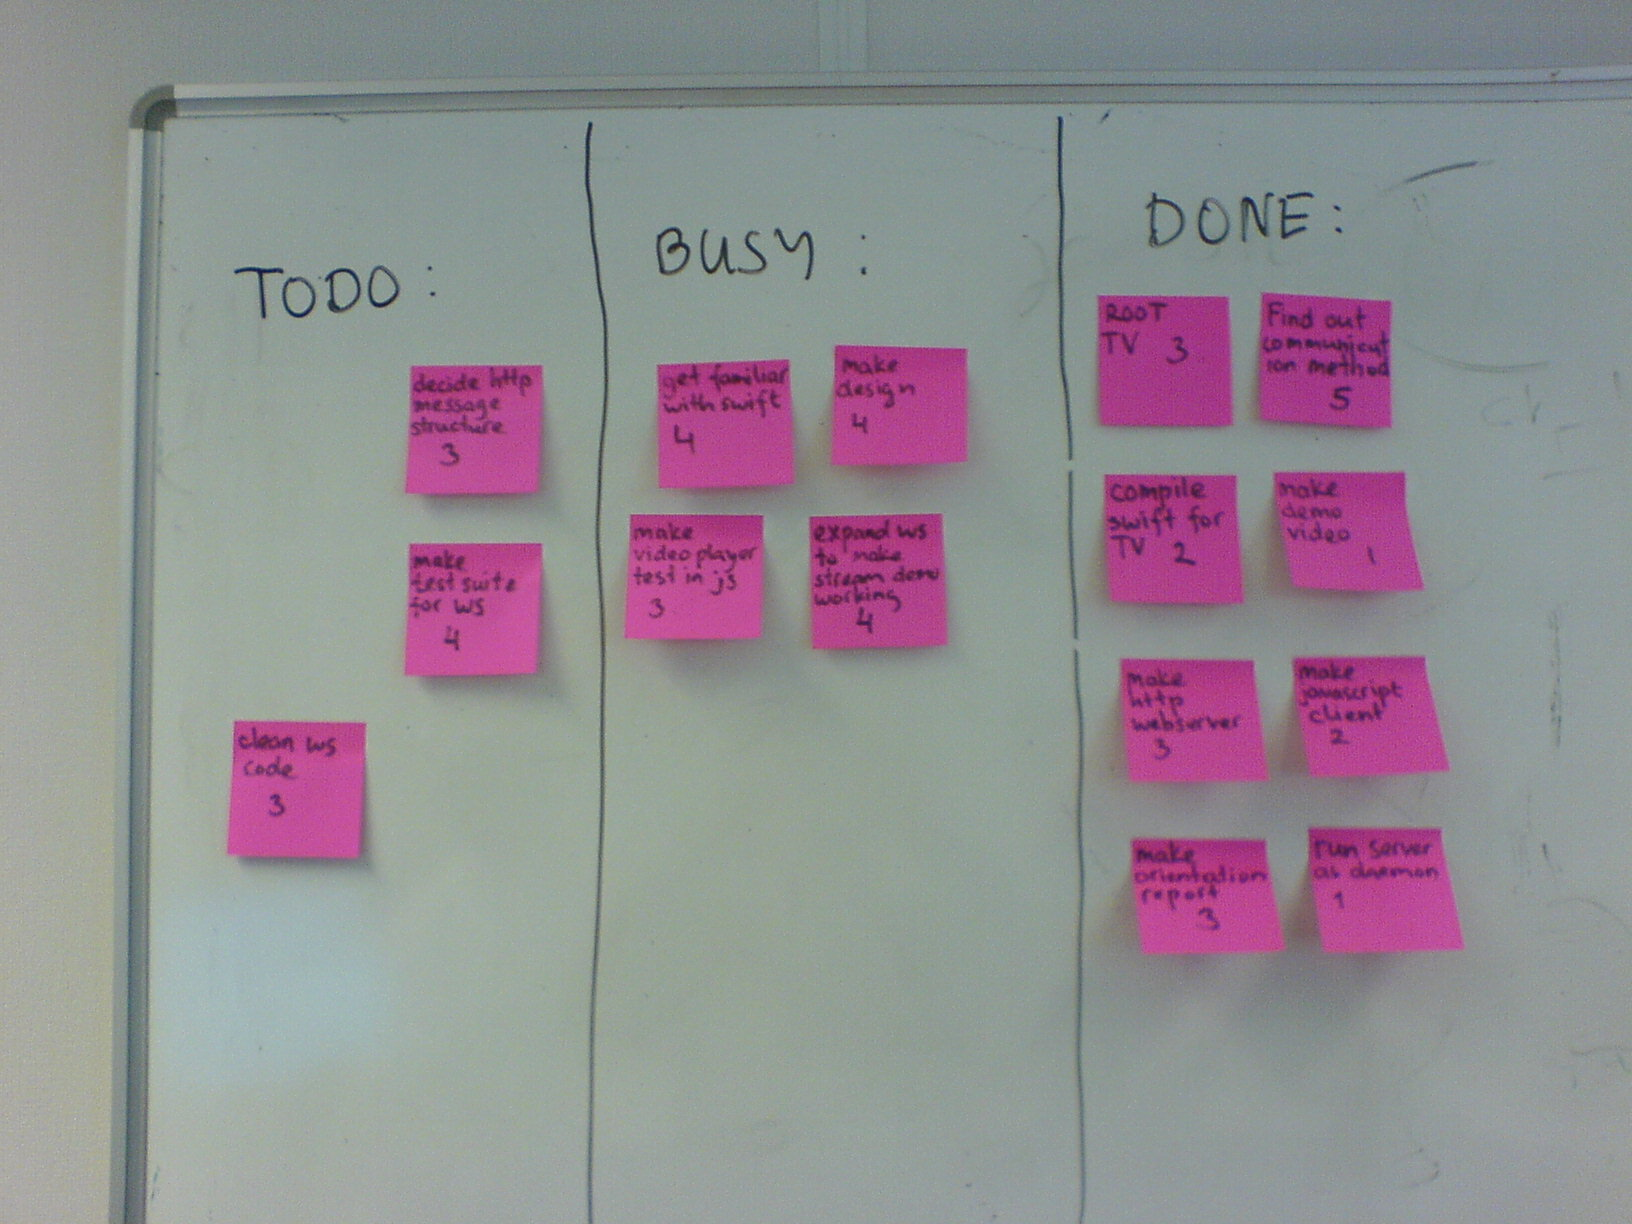
\includegraphics[width=1\textwidth]{Images/process.jpg}}
	\caption{The whiteboard used to keep track of tasks.}
	\label{fig:board}
\end{figure}
\end{center}

\section{Decision taking}
The way we decided to implement certain features was rather simple. We first determined whether it was possible to implement the feature for the TV.
If multiple solutions were proposed by the group, the complexity of the solution and the time it would take to implement it were taken into consideration.
If all conditions were met, we just started to implement as much as possible.

\section{Testing}

We only wrote tests for C++ as this was the core of our application. We made use of the google test library which allowed for easy implementation of unit tests. The tests were developed in parallel with the development of the application which allowed for constant checking for bugs with every change. This way most bugs were immediately discovered and removed as soon as they appeared. Writing the tests also helped making the system robust and able to handle unexpected input and calls without crashing.
\\\\
Every class has its own test class and almost every method has its own tests, usually a trivial test and additionally a couple of tests with unexpected input or unexpected situations. Certain classes, especially DownloadManager, required test cases to call multiple different methods in order to test certain situations. Although this resulted in some relatively long test cases it did guarantee a solid application capable of handling a large range of exceptional situations.
\\\\
We chose not to fully test SearchEngine, the reason being that SearchEngine relies on dispersy and DHT. Both of these services are unreliable when it comes to returning search results, you do not always get the same results and sometimes you get no results. The testing environment requires a fixed return value every time. In order to achieve this we created a mock of the SearchEngine class which has the same functionality as the real SearchEngine except when it comes to searching. The mock always returns the exact same results which are hard coded in the mock. This allowed us to test HttpServer without having to worry about dispersy and DHT returning different values every time.

\section{Problems encountered}
This section focusses on all the important problems we encountered while developing the application for the TV. A brief explanation will be given per problem together with the solution we came up with.
 Some of these solutions were found with the help of the tribler team.

\subsection{Rooting the television}
The first hurdle before we could even start developing was gaining root access to the television. We needed this to be able to install libraries and execute code. Rooting the television should not have been an issue as there are tutorials and an app that roots the television for you from SamyGO\cite{SamyGO}. The problem we ran into is that the televisions we got had a new firmware for which there was no way to root yet.
\\\\
We had a quick look into finding a vulnerability in the new firmware that would allow us to execute arbitrary code and gain root access. We did find a possible vulnerability in ffmpeg, in the part used to decode Matroska video files, but developing an exploit for this would have taken too long as we did not have any experience in this field.
\\\\
Another option was to downgrade the firmware to a previous version that would allow us to use the SamyGO app to gain root access. Samsung has not made the option of downgrading available, it is only possible to upgrade, so we had to trick the TV into thinking it was upgrading while actually it was installing old firmware. It is possible to install new firmware via a USB device which is what we initially tried. We took some old firmware, unpacked it, changed the version numbers inside, repacked it and recalculated the MD5 hash and changed that too so that they would match. Sadly, this is when we found out that the firmware also required a signature from Samsung which is something we did not have. This made downgrading via a USB device impossible.
\\\\
We contacted SamyGO to ask whether there was any way to downgrade to an older firmware. Initially the answer was no but after some prodding they allowed us to make use of a server they had set up which pretends to be the Samsung firmware update server. Apparently the online firmware update did not require a Samsung signature or they had access to it. Either way, we now had a television with an old firmware which allowed us to run the SamyGO app and root the TV.

\subsection{Installing missing dependencies}
Even though the SmartTV runs a linux kernel, not everything was available from the start, so we had to install a great number of packages on the TV.
For this purpose, we used cross-compiling toolchains to build executables compatible with the ARM \cite{arm} processors which resides in the TV. However, we failed
to fully compile some of these packages, of which the Python interpreter is one of the most important. The Python interpreter was needed because the dispersy and DHT modules 
developed by the Tribler team were written in Python. Since we had to use these modules in our application, we also needed to install Python on the TV. 
\\\\
We succeeded in cross-compiling and running the interpreter on the TV, but not in cross-compiling the standard Python-modules we need to run simple Python executables.
Our solution was to emulate the ARMv7 processor with QEMU \cite{qemu}. Within this emulator, we installed a copy of Ubuntu, \cite{ubuntu} which functioned as a binary compatible development platform and with which we were able to install the Python package with the apt tool.
To achieve this, it was also needed to enable networking within QEMU. \cite{qemu-network} Then we copied the binary files to the TV, after which we could succesfully run the Python interpreter together with all its dependencies.
\\\\
Aside from Python, we also installed other applications via QEMU such as bash, sshd etc. to make it easier to work on the TV to accelerate the development.

\subsection{TCP RST packages}
It appeared that the Samsung TV sent TCP RST packages to itself after each HTTP request. TCP RST packages can be distinguished by looking at the fourth flag in the TCP header. This flag is the reset flag, which was activated in our case (see figure \ref{fig:TCP_RST}). Because of this, TCP connections to swift were interrupted each time a RST package was received, because the TCP connection was reset. This was a problem for file streaming, because the connection used by libswift to download the stream was continually interrupted, so the stream could not be played correctly. 
\\\\
We solved this problem by cross-compiling iptables\cite{iptables} for the TV, so we could set up some rules to block these TCP RST packages. This required us to insert several kernel modules. Because this needs to be done each time the TV reboots, we added some rules to the init script of the TV so that these kernel modules are loaded automatically, together with the rules written for iptables (see \hyperref[sec:vusb_init]{appendix}).

\begin{center}
\begin{figure}[h]
	\centering
	\mbox{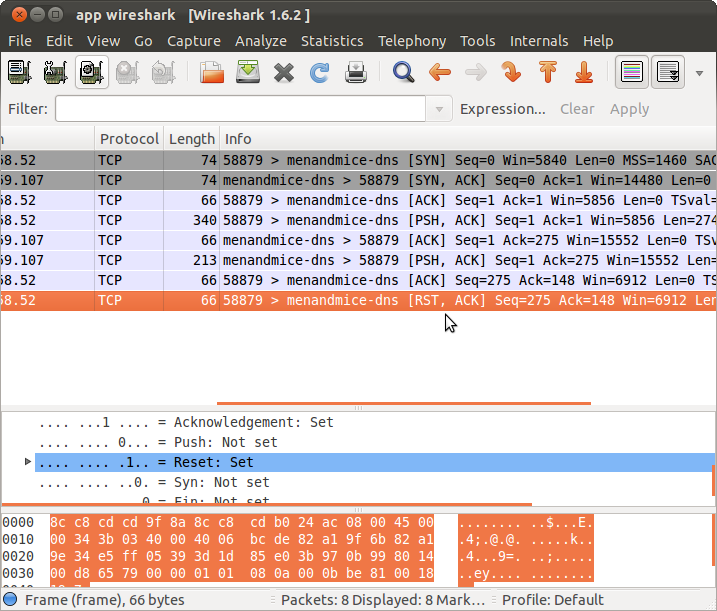
\includegraphics[width=1\textwidth]{Images/tcp_rst.png}}
	\caption{Screenshot of wireshark. The RST package is highlighted in orange. Also, in the lower part of the screen it can be seen that the RST flag is set.}
	\label{fig:TCP_RST}
\end{figure}
\end{center}

\clearpage

\subsection{Fork() and thread problem}
For testing purposes, we used a webserver written in C++ we found on the Internet. We were 
not aware, however, that this webserver was implemented so that it would call the fork() 
method each time a HTTP request was received. We were using p\_threads\cite{thread} to start several libevent\cite{libevent} loops needed for downloading files and p\_threads cannot access data directly within other processes. So we got the problem that the threads were not able to access the correct data.
\\\\
The problem was that fork() creates a new process, which is an exact copy of the parent 
process (See figure \ref{fig:fork_thread}). So all global variables and threads running 
within the process were also copied. Now, each time we tried to access a global variable, we 
noticed that the values of the variables were inconsistent because we were setting and 
reading the wrong variables. Unconsciously, we would set the value of a global variable, but 
read out the value of its copy instead, which has not been set yet. This caused unexpected 
behaviour of our application, on which we spent a lot of time. Strangely enough, this problem 
did not occur when we compiled and ran the program for our own pc\textquotesingle s, but only when we tried it on the TV.
\\\\
A solution is to implement pipes, which provide inter-process communication. With this, threads are able to access data outside their own process scope so the correct variables can be read. 
\\\\
In the end, we solved this problem by implementing a new HTTP server by ourselves, which makes use of the libevent library. This version of the webserver does not call the fork() method, so we did not have the problem of threads not being able to access the same data.

\begin{center}
\begin{figure}[h]
	\centering
	\mbox{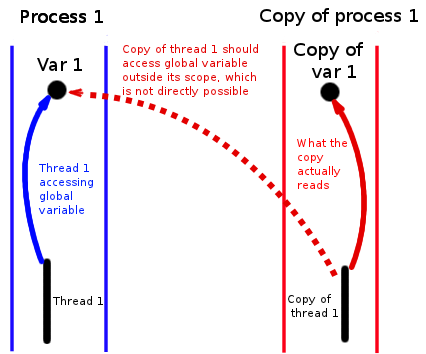
\includegraphics[width=0.8\textwidth]{Images/fork-thread.png}}
	\caption{The fork()-thread problem. Threads are accessing the wrong data.}
	\label{fig:fork_thread}
\end{figure}
\end{center}

\subsection{Communication between JavaScript and C++}
One of the first issues we encountered was how to link JavaScript to C++ so that we could call C++ functions from within the GUI and get return values back. Initially we wanted to use a language binder like SquirrelFish or a JavaScript engine for C++ like google V8. However due to the restrictions set by Samsung you are forced to develop the JavaScript app using their SDK and it is impossible to add any additional tools. This left us with the standard JavaScript functionality and the Samsung API. As Samsung does not allow any development outside of JavaScript there was no support for calling C++ applications in their API either. The only remaining option was to use HTTP requests which is part of the standard functionality in JavaScript.
\\\\
This did require us to be running an HTTP server in C++ which needs to be running before the Javascript app had even been started. Newer version of the firmware also support HTML5 and websockets. This would allow for better two way communication betweem JavaScript and C++ rather than JavaScript constantly polling the HTTP server when it needs updates. The downside of this newer firmware is that there is no known way to gain root access yet which is why we could not use it.

\subsection{Starting the HTTP server}

Sending HTTP requests was the only way to communicate between JavaScript and C++ but there 
was no way to start the HTTP server in C++ from JavaScript. We needed to start the HTTP 
server as soon as the television was switched on. In principle it would have been possible 
to run the HTTP server as a daemon on start-up but it was not possible to edit the Samsung 
init scripts. SamyGO, however, also uses init scripts when they root the television which 
we could edit. Now whenever you root the television using SamyGO you also automatically 
start running the HTTP server for our application. This does mean that running SamyGO is 
required to be able to use our application.

\subsection{USB write speed}

Initially we were planning to use a USB storage device to store downloads and streams. 
As it turned out, the write speed of the TV to the USB device was so slow that streaming 
was not possible when using it to store the data. Downloading to an external USB device was 
also so slow that it was not practical to do so. This left us with only the internal 
memory of the TV for downloads and streams which is a very limited amount. This caused 
large files to be impossible to stream as they would fill the memory and cause the TV to 
hang. The maximum file size that can be downloaded is also very low as a result of this.

\chapter{Conclusion}
Based on the final product of the project it is safe to say that peer-to-peer applications involving streaming, downloading and uploading of files is possible on smart TV's. Due to hardware limitations the application was never able to reach its full potential but the results are very promising for future televisions with better hardware. Dispite the hardware issues, the technology does work which makes our application is the first fourth generation peer-to-peer file sharing application in the world.

Another important aspect as to whether more advanced applications will be developed for televisions is the amount of freedom manufacturers are willing to give to developers. As it stands, television manufacturers seem very weary of giving any access to their TV's, which is very understandable from a security point of view. However, if the full potential of the smart TV is to be reached, developers must be given full access to develop advanced programs or else the smart TV will remain a gimmick with limited functionality.
\chapter{Recommendations}
\label{sec:recommendations}


\appendix
\chapter{UML Models}

\section{Business Class Diagram}

\begin{center}
\begin{figure}[h!]
\scalebox{0.65}{
\begin{tikzpicture}
%\begin{umlpackage}{p}
%\begin{umlpackage}{sp1}

\umlclass[x=-5]{Sendable}{
  - trackers : list<tracker> \\
  - seeders  : list<seeder> \\
  - speed    : double
}{
  + start() : void \\
  + stop() : void \\
  + pause() : void \\
  + resume() : void
}

\umlclass[x=3]{FileManager}{
  - list<File>
}{
  + remove(File file) : void \\
  + add(File file) : File \\
  + rename(File file) : File \\
  + sort() : void \\
  + search(File file) : list<File> \\
}

\umlclass[x=3, y=-6]{File}{
  - name : String \\
  - date : String \\
  - extension : String \\
  - size : double \\
  - visible : bool \\
}{
  + setVisibility(bool value) : void \\
  + isVisible() : bool \\
  + setName(String name) : void \\
  + getSize() : double \\
  + getDate() : String \\
  + getName() : String
}

\umlclass[x=4, y=-11]{Media}{
  - length : double \\
}{}

\umlclass[x=-7, y=-4]{Download}{
  - percentage : double
}{}

\umlclass[x=-3, y=-4]{Upload}{
  - amount : double
}{}

\umlclass[x=-5, y=-6]{Stream}{
  - length : double
}{}

\umlclass[x=-5, y=-10.5]{DownloadManager}{
  - downloaded : double \\
  - uploaded : double \\
  - downloads : list<Download> \\
  - uploads : list<Uploads>
}{
  + startDownload(String link) : void \\
  + stopDownload(String link) : void \\
  + pauseDownload(String link) : void \\
  + resumeDownload(String link) : void \\
  + startUpload(String name) : void \\
  + stopUpload(String name) : void
}

\umlclass[x=2, y=-14]{MediaPlayer}{
}{
  + open(Media file) : void \\
  + open(Stream stream) : void
}

\umlaggreg[mult1=1, mult2=1, pos=0.8, angle1=30, angle2=60]{Sendable}{File}
\umlaggreg[mult1=1, mult2=*]{FileManager}{File}

\umlinherit{Download}{Sendable}
\umlinherit{Upload}{Sendable}
\umlinherit{Stream}{Sendable}

\umlinherit{Media}{File}

\umlVHVaggreg[mult1=1, mult2=*]{DownloadManager}{Upload}
\umlVHVaggreg[mult1=1, mult2=*]{DownloadManager}{Download}

\umlVHassoc{MediaPlayer}{Stream}
\umlVHassoc{Media}{MediaPlayer}

\end{tikzpicture}}
\caption{Part of the class diagram. This part only shows the business classes comprehensible for end-users.}
\label{fig:business_class}
\end{figure}
\end{center}

\section{Use Case Dynamic Models}
\label{sec:req_dynamic_models}
\begin{figure}[h!]
\scalebox{1}{
\begin{tikzpicture}
\begin{umlseqdiag}
\umlactor{User}
\umlobject[x=5]{Samsung App Interface}
\umlobject[x=10]{DownloadManager}
\begin{umlcall}[op={goToSettings()}, with return, padding=3]{User}{Samsung App Interface}
\begin{umlcall}[op={getSettings()}, with return]{Samsung App Interface}{DownloadManager}
\end{umlcall}
\end{umlcall}
\begin{umlcall}[op={setSpeeds(dspeed, uspeed)}, padding=3, with return]{User}{Samsung App Interface}

\begin{umlcall}[op={setSpeeds(dspeed, uspeed)}, padding=3, with return]{Samsung App Interface}{DownloadManager}
\end{umlcall}
\end{umlcall}
\end{umlseqdiag}
\end{tikzpicture}
}
\caption{Use Case 1: Limit upload/download speeds.}
\label{fig:req_seq1}
\end{figure}

\begin{figure}[h!]
\scalebox{0.8}{
\begin{tikzpicture}
\begin{umlseqdiag}
\umlactor{User}
\umlobject{Samsung App Interface}
\umlobject{FileManager}
\umlobject{MediaPlayer}
\umlmulti{File}

\begin{umlcall}[op={browse}, with return, padding=3]{User}{Samsung App Interface}
	\begin{umlcall}[op={getFiles()}, with return, padding=3]{Samsung App Interface}{FileManager}
		\begin{umlcall}[op={get()}, with return, padding=3]{FileManager}{File}
		\end{umlcall}
	\end{umlcall}
\end{umlcall}

\begin{umlfragment}[type=alt, label=Update, inner xsep=5]
\begin{umlcall}[op={update}, with return]{User}{Samsung App Interface}
	\begin{umlcall}[op={update(int file\_id)}, with return]{Samsung App Interface}{FileManager}
		\begin{umlcall}[op={update()}, with return]{FileManager}{File}
		\end{umlcall}
	\end{umlcall}
\end{umlcall}

\umlfpart [Delete]
\begin{umlcall}[op={delete}, with return]{User}{Samsung App Interface}
	\begin{umlcall}[op={delete(int file\_id)}, with return]{Samsung App Interface}{FileManager}
		\begin{umlcall}[op={destroy()}, with return]{FileManager}{File}
		\end{umlcall}
	\end{umlcall}
\end{umlcall}

\umlfpart[Move]
\begin{umlcall}[op={move}, with return]{User}{Samsung App Interface}
	\begin{umlcall}[op={move(string location, int file\_id)}, with return]{Samsung App Interface}{FileManager}
		\begin{umlcall}[op={changeLocation(string location)}, with return]{FileManager}{File}
		\end{umlcall}
	\end{umlcall}
\end{umlcall}

\umlfpart[Play]
\begin{umlcall}[op={play}, with return]{User}{Samsung App Interface}
	\begin{umlcall}[op={play(int file\_id)}, with return]{Samsung App Interface}{MediaPlayer}
		\begin{umlcall}[op={play()}, with return]{MediaPlayer}{File}
		\end{umlcall}
	\end{umlcall}
\end{umlcall}

\end{umlfragment}
\end{umlseqdiag}
\end{tikzpicture}
}
\caption{Use Cases 2 to 6: Basic browsing and file manipulation}
\label{fig:req_seq2}
\end{figure}

\begin{figure}[h!]
\scalebox{0.9}{
\begin{tikzpicture}
\begin{umlseqdiag}
\umlactor[y=1]{User}
\umlobject[y=1, x=3]{Samsung App Interface}
\umlobject[y=1, x=7]{FileManager}
\umlmulti[y=1, x=12]{File}

\begin{umlcall}[op={change visbility}]{User}{Samsung App Interface}
\end{umlcall}

\begin{umlfragment}[type=alt, label=visible, inner xsep=5]

\begin{umlcall}[op={changeVisibility(file, true)}, with return]{Samsung App Interface}{FileManager}
		\begin{umlcall}[op={visible(true)}, with return]{FileManager}{File}
		\end{umlcall}
\end{umlcall}

\umlfpart[invisible]

\begin{umlcall}[op={changeVisibility(file, false)}, with return]{Samsung App Interface}{FileManager}
		\begin{umlcall}[op={visible(false)}, with return]{FileManager}{File}
		\end{umlcall}
\end{umlcall}

\end{umlfragment}

\end{umlseqdiag}
\end{tikzpicture}
}
\caption{Use Case 7: Change File Visibility}
\label{fig:req_seq3}
\end{figure}

\begin{figure}[h!]
\scalebox{0.8}{
\begin{tikzpicture}
\begin{umlseqdiag}
\umlactor{User}
\umlobject{Samsung App Interface}
\umlobject{FileManager}
\umlobject{DownloadManager}
\umlmulti{File}

\begin{umlcall}[op={goToSearch}, with return, padding=3]{User}{Samsung App Interface}
\end{umlcall}

	\begin{umlfragment}[type=alt, label=Local, inner xsep=5]
		\begin{umlcall}[op={searchLocal(file)}, with return]{User}{Samsung App Interface}
			\begin{umlcall}[op={search(file)}, with return]{Samsung App Interface}{FileManager}
				\begin{umlcall}[op={get()}, with return]{FileManager}{File}
				\end{umlcall}	
			\end{umlcall}
		\end{umlcall}

	\umlfpart [Online]
\begin{umlcall}[op={searchOnline(file)}, with return]{User}{Samsung App Interface}
	\begin{umlcall}[op={search(file)}, with return]{Samsung App Interface}{DownloadManager}
		\begin{umlcall}[op={get()}, with return]{DownloadManager}{File}
		\end{umlcall}
	\end{umlcall}
\end{umlcall}

	
	\end{umlfragment}

\end{umlseqdiag}
\end{tikzpicture}
}
\caption{Use Cases 8 to 10: Search.}
\label{fig:req_seq4}
\end{figure}

\begin{figure}[h!]
\scalebox{1}{
\begin{tikzpicture}
\begin{umlseqdiag}
\umlactor{User}
\umlobject{Samsung App Interface}
\umlobject{DownloadManager}
\umlobject{Stream}

\begin{umlcall}[op={play}]{User}{Samsung App Interface}
\end{umlcall}

\begin{umlcall}[op={playStream(string tracker)}]{Samsung App Interface}{DownloadManager} 
	\begin{umlcall}[op={start()}]{DownloadManager}{Stream} 
	\end{umlcall}
\end{umlcall}

\end{umlseqdiag}
\end{tikzpicture}
}
\caption{Use Case 11: Stream File.}
\label{fig:req_seq5}
\end{figure}

\begin{figure}[h!]
\scalebox{1}{
\begin{tikzpicture}
\begin{umlseqdiag}
\umlactor{User}
\umlobject{Samsung App Interface}
\umlobject{DownloadManager}

\begin{umlcall}[op={download}]{User}{Samsung App Interface}  
\end{umlcall}

\umlcreatecall[class=Download]{Samsung App Interface}{download} 

\begin{umlcall}[op={add(download)}]{Samsung App Interface}{DownloadManager} 
	\begin{umlcall}[op={start()}]{DownloadManager}{download} 
	\end{umlcall} 
\end{umlcall}

\end{umlseqdiag} 
\end{tikzpicture}
}
\caption{Use Case 12: Download File.}
\label{fig:req_seq6}
\end{figure}

\begin{figure}[h!]
\scalebox{1}{
\begin{tikzpicture}
\begin{umlseqdiag}
\umlactor{User}
\umlobject{Samsung App Interface}
\umlobject{FileManager}

	\begin{umlcall}[op={sortName()}, with return]{User}{Samsung App Interface}
		\begin{umlcall}[op={sortName()}, with return]{Samsung App Interface}{FileManager}
		\end{umlcall}
	\end{umlcall}
	
\begin{umlfragment}[type=alt, label=Size, inner xsep=5]
	\begin{umlcall}[op={sortSize(), with return}]{User}{Samsung App Interface}
		\begin{umlcall}[op={sortSize()}, with return]{Samsung App Interface}{FileManager}
		\end{umlcall}
	\end{umlcall}
		
	\umlfpart [Type]
	\begin{umlcall}[op={sortType(), with return}]{User}{Samsung App Interface}
		\begin{umlcall}[op={sortType()}, with return]{Samsung App Interface}{FileManager}
		\end{umlcall}
	\end{umlcall}
		
	\umlfpart [Date]
	\begin{umlcall}[op={sortDate(), with return}]{User}{Samsung App Interface}
		\begin{umlcall}[op={sortDate()}, with return]{Samsung App Interface}{FileManager}
		\end{umlcall}
	\end{umlcall}
\end{umlfragment}

\end{umlseqdiag}
\end{tikzpicture}
}
\caption{Use Cases 13 to 17: Sort Files.}
\label{fig:req_seq7}
\end{figure}

\clearpage

\section{Class diagram}

\begin{center}
\begin{figure}[h!]
\scalebox{1}{
\begin{tikzpicture}
%\begin{umlpackage}{p}
%\begin{umlpackage}{sp1}

\umlclass[x=-10]{Download}{
  - tracker : char* \\
  - id : int \\
  - seeders : int \\
  - peers : int \\
  - ratio : double \\
  - download\_speed : double \\
  - size : double \\
  - upload\_speed : double \\
  - download\_percentage : double \\
  - upload\_amount : double \\
  - is\_visible : bool \\
  - status : Status
}{
  + start() : void \\
  + resume() : void \\
  + pause() : void \\
  + setVisible(bool visible) : void
}

\umlclass[x=-1.5, y=-12]{Stream}{
  - tracker : char*
}{
  + start() : void \\
  + resume() : void \\
  + pause() : void \\
  + stop() : void
}
\umlclass[x=-10, y=-12]{DownloadManager}{
  - downloaded : double \\
  - uploaded : double \\
  - downloads : list<Download> \\
  - uploads : list<Download> \\
}{
  + getInstance() : void \\
  + startStreaming(string tracker) : void \\
  + stopStreaming() : void \\
  + add(Download download) : void \\
  + setVisible(Download download) : void \\
  + setUnvisible(Download download) : void \\
  + resumeDownload(Download download) : void \\
  + removeFromList(int download\_id) : void \\
  + removeFromDisk(int download\_id) : void \\
  + setSpeed(double dspeed, double uspeed)
}

\umlclass[x=-3, y=-6]{HttpServer}{
}{
  + InstallHTTPGateway() : bool \\
  + sendResponse() : void \\
  + sendXMLResponse() : void \\
  + handle\_request(struct evhttp\_request *req, void *arg) : void \\
}

\umlclass[x=-0.5, y = 2]{SearchEngine}{
}{
  + search(char* filename) : void \\
  + getResults() : char*
}

\umlVHassoc[mult1=1, mult2=*]{HttpServer}{Download}
\umlassoc[mult1=1, mult2=1]{HttpServer}{DownloadManager}
\umlVHassoc[mult1=1, mult2=1]{SearchEngine}{HttpServer}

\umlaggreg[mult1=1, mult2=*]{DownloadManager}{Download}
\umlaggreg[mult1=1, mult2=1]{DownloadManager}{Stream}

\end{tikzpicture}}
\caption{Class diagram of the webserver subsystem.}
\label{fig:class_server}
\end{figure}
\end{center}

\section{Dynamic models}

\begin{figure}[h!]
\scalebox{1}{
\begin{tikzpicture}
\begin{umlseqdiag}
\umlactor{Samsung SDK client}
\umlobject[x=5]{HttpServer}
\umlobject[x=8]{DownloadManager}
\begin{umlcall}[op={sendRequest(add download)}, with return, padding=3]{Samsung SDK client}{HttpServer}
	\begin{umlcall}[op={add(download)}, with return, padding=3]{HttpServer}{DownloadManager}
		\umlcreatecall[class=Download]{DownloadManager}{download}
		\begin{umlcall}[op={setStatus(READY)}, padding=3]{DownloadManager}{download}
		\end{umlcall}
		\begin{umlcall}[op={push(download)}, padding=3]{DownloadManager}{DownloadManager}
		\end{umlcall}
	\end{umlcall}
\end{umlcall}
\end{umlseqdiag}
\end{tikzpicture}
}
\label{fig:seq1}
\caption{Add download}
\end{figure}

\begin{figure}[h!]
\scalebox{0.7}{
\begin{tikzpicture}
\begin{umlseqdiag}
\umlactor{Samsung SDK client}
\umlobject[x=5]{HttpServer}
\umlobject[x=8]{DownloadManager}
\umlobject[x=12]{Download}
\umlobject[x=18]{Swift}
\begin{umlcall}[op={sendRequest(start download)}, with return, padding=3]{Samsung SDK client}{HttpServer}
	\begin{umlcall}[op={start(download)}, with return, padding=3]{HttpServer}{DownloadManager}
		\begin{umlcall}[op={get(download)}, padding=3]{DownloadManager}{DownloadManager}
		\end{umlcall}
		
		\begin{umlcall}[op={start(download)}, with return, padding=3]{DownloadManager}{Download}
			\begin{umlcall}[op={setStatus(DOWNLOADING)}, padding=3]{Download}{Download}
			\end{umlcall}
			
			\begin{umlcall}[op={getTrackerAddress()}, with return, padding=3]{Download}{Swift}
			\end{umlcall}
			
			\begin{umlcall}[op={getRootHash()}, with return, padding=3]{Download}{Swift}
			\end{umlcall}
			
			\begin{umlcall}[op={Open(filename, root\_hash, tracker\_address)}, padding=3]{Download}{Swift}
			\end{umlcall}
			
		\end{umlcall}
		
		
	\end{umlcall}
\end{umlcall}
\end{umlseqdiag}
\end{tikzpicture}
}
\caption{Start download}
\label{fig:seq2}
\end{figure}

\begin{figure}[h!]
\scalebox{0.7}{
\begin{tikzpicture}
\begin{umlseqdiag}
\umlactor{Samsung SDK client}
\umlobject[x=5]{HttpServer}
\umlobject[x=8]{DownloadManager}
\umlobject[x=12]{Download}
\umlobject[x=18]{Swift}
\begin{umlcall}[op={sendRequest(pause download)}, with return, padding=3]{Samsung SDK client}{HttpServer}
	\begin{umlcall}[op={pause(download)}, with return, padding=3]{HttpServer}{DownloadManager}
		\begin{umlcall}[op={get(download)}, padding=3]{DownloadManager}{DownloadManager}
		\end{umlcall}
		
		\begin{umlcall}[op={pause(download)}, with return, padding=3]{DownloadManager}{Download}
			\begin{umlcall}[op={setStatus(PAUSED)}, padding=3]{Download}{Download}
			\end{umlcall}
			
			\begin{umlcall}[op={getID()}, padding=3]{Download}{Download}
			\end{umlcall}
			
			\begin{umlcall}[op={Checkpoint(id)}, padding=3]{Download}{Swift}
			\end{umlcall}
			
			\begin{umlcall}[op={Close(id)}, padding=3]{Download}{Swift}
			\end{umlcall}
			
		\end{umlcall}
		
		
		
	\end{umlcall}
\end{umlcall}
\end{umlseqdiag}
\end{tikzpicture}
}
\caption{Pause download}
\label{fig:seq3}
\end{figure}

\begin{figure}[h!]
\scalebox{0.7}{
\begin{tikzpicture}
\begin{umlseqdiag}
\umlactor{Samsung SDK client}
\umlobject[x=5]{HttpServer}
\umlobject[x=12]{DownloadManager}
\umlobject[x=15]{Download}
\umlobject[x=18]{Swift}
\begin{umlcall}[op={sendRequest(setUnvisible download)}, with return, padding=3]{Samsung SDK client}{HttpServer}
	\begin{umlcall}[op={setUnvisible(download)}, with return, padding=3]{HttpServer}{DownloadManager}
		\begin{umlcall}[op={get(download)}, padding=3]{DownloadManager}{DownloadManager}
		\end{umlcall}

			\begin{umlcall}[op={getID()}, padding=3]{DownloadManager}{Download}
			\end{umlcall}
					
		\begin{umlcall}[op={removeFromList(id)}, with return, padding=3]{DownloadManager}{Download}
			\begin{umlcall}[op={setVisible(false)}, padding=3]{Download}{Download}
			\end{umlcall}
			
			\begin{umlcall}[op={Close(id)}, padding=3]{Download}{Swift}
			\end{umlcall}
			
		\end{umlcall}
		
	\end{umlcall}
\end{umlcall}
\end{umlseqdiag}
\end{tikzpicture}
}
\caption{Set unvisible}
\label{fig:seq4}
\end{figure}

\begin{figure}[h!]
\scalebox{0.7}{
\begin{tikzpicture}
\begin{umlseqdiag}
\umlactor{Samsung SDK client}
\umlobject[x=5]{HttpServer}
\umlobject[x=8]{DownloadManager}
\umlobject[x=12]{Download}
\umlobject[x=18]{Swift}
\begin{umlcall}[op={sendRequest(setVisible download)}, with return, padding=3]{Samsung SDK client}{HttpServer}
	\begin{umlcall}[op={setVisible(download)}, with return, padding=3]{HttpServer}{DownloadManager}
		\begin{umlcall}[op={get(download)}, padding=3]{DownloadManager}{DownloadManager}
		\end{umlcall}
		
		\begin{umlcall}[op={resumeDownload(download)}, with return, padding=3]{DownloadManager}{Download}
			
			\begin{umlcall}[op={getTrackerAddress()}, with return, padding=3]{Download}{Swift}
			\end{umlcall}
			
			\begin{umlcall}[op={getRootHash()}, with return, padding=3]{Download}{Swift}
			\end{umlcall}
			
			\begin{umlcall}[op={Open(filename, root\_hash, tracker\_address)}, padding=3]{Download}{Swift}
			\end{umlcall}
			
		\end{umlcall}
		
	\end{umlcall}
\end{umlcall}
\end{umlseqdiag}
\end{tikzpicture}
}
\caption{Set visible}
\label{fig:seq5}
\end{figure}

\begin{figure}[h!]
\scalebox{0.6}{

\begin{tikzpicture}
\begin{umlseqdiag}
\umlactor{Samsung SDK client}
\umlobject[x=5]{HttpServer}
\umlobject[x=10]{DownloadManager}
\umlobject[x=14]{Stream}

\begin{umlcall}[op={sendRequest(startStream)}, with return, padding=3]{Samsung SDK client}{HttpServer}
	
		\begin{umlcall}[op={startStreaming(tracker\_address)}, with return, padding=3] 	
	{HttpServer}{DownloadManager}
	
	
			\begin{umlcall}[op={setTracker(tracker\_address)}, with return, padding=3]
{DownloadManager}{Stream}
		
			\end{umlcall}
		
			\begin{umlcall}[op={start()}, with return, padding=3]{DownloadManager}{Stream}
			
				\begin{umlcall}[op={evtimer\_assign(event, evbase, closeCallback, this)}, 
padding=3]{Stream}{Stream}
			
				\end{umlcall}
			
				\begin{umlcall}[op={evtimer\_add(event, swift::tint2tv(TINT\_SEC)}, 
padding=3]{Stream}{Stream}
			
				\end{umlcall}
			
			
				\begin{umlcall}[op={event\_base\_dispatch(evbase)}, padding=3]{Stream}
{Stream}
		
				\end{umlcall}
		
			\end{umlcall}
		
	\end{umlcall}
	
\end{umlcall}
\end{umlseqdiag}

\end{tikzpicture}
}
\caption{Start streaming}
\label{fig:seq6}
\end{figure}

\begin{figure}[h!]
\scalebox{0.7}{

\begin{tikzpicture}
\begin{umlseqdiag}
\umlactor{Samsung SDK client}
\umlobject[x=5]{HttpServer}
\umlobject[x=10]{DownloadManager}
\umlobject[x=14]{Stream}

\begin{umlcall}[op={sendRequest(stopStream)}, with return, padding=3]{Samsung SDK client}{HttpServer}
	
		\begin{umlcall}[op={stopStreaming()}, with return, padding=3] 	
	{HttpServer}{DownloadManager}
	
			\begin{umlcall}[op={stop()}, with return, padding=3]{DownloadManager}{Stream}
			
				\begin{umlcall}[op={evtimer\_del(swift::Channel::evbase)}, padding=3]{Stream}{Stream}
		
				\end{umlcall}
		
			\end{umlcall}
		
		\end{umlcall}
	
\end{umlcall}
\end{umlseqdiag}

\end{tikzpicture}
}
\caption{Stop streaming}
\label{fig:seq7}
\end{figure}

\clearpage

\chapter{SIG feedback}
\label{sec:sig}
\section{First feedback}
De code van het systeem scoort vier sterren op ons onderhoudbaarheidsmodel, wat betekent dat de code bovengemiddeld onderhoudbaar is. De hoogste score is niet behaald door een lagere score voor Unit Size en de Unit Complexity.

Voor Unit Size wordt er gekeken naar het percentage code dat bovengemiddeld lang is. Het opsplitsen van dit soort methodes in kleinere stukken zorgt ervoor dat elk onderdeel makkelijker te begrijpen, te testen en daardoor eenvoudiger te onderhouden wordt. Binnen de extreem lange methodes in dit systeem, zoals bijvoorbeeld de 'HttpServer::handleRequest'-methode, zijn aparte stukken functionaliteit te vinden welke ge-refactored kunnen worden naar aparte methodes. Commentaarregels zoals bijvoorbeeld '// Message will look like: "/pause:roothash"' en ' // Some garbage collecting.' zijn een goede indicatie dat er een autonoom stuk functionaliteit te ontdekken is. Ook aan de kant van de 'swift\_p2ptv' zijn langere methoden te vinden, bijvoorbeeld 'ScenePlayer.prototype.handleKeyDown'. In dit type methoden is het aan te raden om de afhandeling van een bepaalde 'keyCode' in een aparte methode te zetten, dit maak het makkelijker om de afzonderlijke stukken functionaliteit te begrijpen en te testen. Het is aan te raden kritisch te kijken naar de langere methodes binnen dit systeem en deze waar mogelijk op te splitsen.

Voor Unit Complexity wordt er gekeken naar het percentage code dat bovengemiddeld complex is. Ook hier geldt dat het opsplitsen van dit soort methodes in kleinere stukken ervoor zorgt dat elk onderdeel makkelijker te begrijpen, makkelijker te testen en daardoor eenvoudiger te onderhouden wordt. In dit geval komen de meest complexe methoden ook naar voren als de langste methoden, waardoor het oplossen van het eerste probleem ook dit probleem zal verhelpen.

Over het algemeen scoort de code bovengemiddeld, hopelijk lukt het om dit niveau te behouden tijdens de rest van de ontwikkelfase. Als laatste nog de opmerking dat er geen (unit)test-code is gevonden in de code-upload. Het is sterk aan te raden om in ieder geval voor de belangrijkste delen van de functionaliteit automatische tests gedefinieerd te hebben om ervoor te zorgen dat eventuele aanpassingen niet voor ongewenst gedrag zorgen.

\chapter{Scripts}
These scripts are already available in the TV when it is rooted. These files are provided by the SamyGO community and are loaded at startup. We edited these files and added the code snippets below to start certain applications and set up certain rules.

\subsection{01\_01\_catch\_crap.init}
\scalebox{0.6}{
\lstinputlisting{Images/01_01_catch_crap.init}
}

\subsection{02\_04\_vusb.init}
\label{sec:vusb_init}
\scalebox{0.6}{
\lstinputlisting{Images/02_04_vusb.init}
}

\chapter{Terms of reference}
\label{sec:terms}
\includepdf[pages={1-2}]{Images/terms.pdf}

\chapter{Orientation Report}
\label{sec:orientation}
\includepdf[pages={1-13}]{Images/orientation.pdf}


\end{document}
